\documentclass[UTF8]{ctexart}
\usepackage{xcolor}      %代码着色宏包
\usepackage{listings}
\usepackage{graphicx}
\definecolor{mygreen}{rgb}{0,0.6,0}
\definecolor{mygray}{rgb}{0.5,0.5,0.5}
\definecolor{mymauve}{rgb}{0.58,0,0.82}
\lstset{ %
backgroundcolor=\color{white},   % choose the background color
basicstyle=\footnotesize\ttfamily,        % size of fonts used for the code
columns=fullflexible,
breaklines=true,                 % automatic line breaking only at whitespace
captionpos=b,                    % sets the caption-position to bottom
tabsize=4,
commentstyle=\color{mygreen},    % comment style
escapeinside={\%*}{*)},          % if you want to add LaTeX within your code
keywordstyle=\color{blue},       % keyword style
stringstyle=\color{mymauve}\ttfamily,     % string literal style
frame=single,
rulesepcolor=\color{red!20!green!20!blue!20},
% identifierstyle=\color{red},
language=c,
}

\usepackage{amsmath}
\title{lab1:实验报告}
\author{学号:PB19111675 姓名:德斯别尔}
\date{\today}
\begin{document}
\maketitle
\section{Romberg 积分}
Romberg积分方法的基本思想是采用复化梯形求积分法不断折半步长的过程中,在积 分结果中加入事后误差估计值进行补偿使积分计算的收敛加速。
\subsection{Romberg 计算公式}
\[ R_{1,1}=\frac{(f(a)-f(b))*h}{2}, \quad h=b-a \]
\[ R_{k,j}=R_{k,j-1}+\frac{R_{k,j-1}-R_{k-1,j-1}}{4^{j-1}-1}, \quad k=2,3,\dots \]
对每个 k,j 从2做到k, 一直做到 $ | R_{k,k}-R_{k-1,k-1} | $ 小于给定控制精度时停止计算。 
\subsection{实验题目}
\paragraph{chapter6.8} $I(ln x) = \int_1^2 {lnx} \,{\rm d}x $, 取 $ \epsilon =10^{-4} , h=1 $ ,试用Romberg公式计算积分直到
\[| R_{k,k}-R_{k-1,k-1} | < \epsilon \]
时停止,并做出Romberg 积分数值表。
\subsection{实验代码}
实验代码如下,是使用C语言完成的。
\lstset{language=C}
\begin{lstlisting}

	#include<stdio.h>
	#include<math.h>
	
	double f(double x)
	{
		return log(x);
	}
	double H(double a, double b, double k)
	{
		return (b-a) / pow(2, k - 1);
	}
	double k_sum(double a, double b, int k)
	{
		double sum = 0;
		for (int i = 1; i <= pow(2, k - 2); i++)
		{
			sum = sum + f(a + (2 * i - 1) * H(a,b,k));
		}
		return sum;
	}
	double romberg(double a, double b, double eps)
	{
		int n = 1, k, j, i;
		double R[10][10];
		R[1][1] = (f(a) + f(b)) * (b - a) / 2;
		for (k = 2;; k++)
		{
			R[k][1] = (R[k - 1][1] + H(a, b, k - 1) * k_sum(a, b, k)) / 2;
			for (j = 2; j <= k; j++)
			{
				R[k][j] = R[k][j - 1] + (R[k][j - 1] - R[k - 1][j - 1]) / (pow(4, j - 1) - 1);
			}
			if (fabs(R[k][k] - R[k - 1][k - 1]) < eps)
				break;
		}
		printf("Romberg积分数值表如下:\n");
		for (i = 1; i <= k; i++)
		{
			for (j = 1; j <= i; j++)
				printf("%f ", R[i][j]);
			printf("\n");
		}
		return R[k][k];
	}
	int main(void)
	{
		double a = 1, b = 2, eps = 0.0001;
		printf("故该函数的结果为:%f\n", romberg(a, b, eps));
		return 0;
	}
	
\end{lstlisting}
\subsection{输出结果}
\begin{figure*}[htbp]
	\begin{center}
	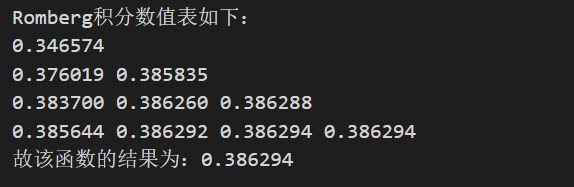
\includegraphics[width=0.85\textwidth]{result.png}
	\end{center}
	\caption{result}
\end{figure*} 
输出结果为:0.386294
\subsection{实验总结}
	第一次使用 \LaTeX 所呈现的结果虽然还不尽人意,但也已经让我十分惊喜并且喜欢上这种排版格式了,在以后的学习过程中我要多加使用 \LaTeX 来对这个工具更加了解。
	同时也算是真正第一次在计算机上使用计算方法的知识,这让我意识到在计算方法这门课程中学习到的知识是多么重要多么实用,我应该更认真地学习这门课程。
\end{document}